\documentclass[journal]{IEEEtran}

\usepackage{cite}
\usepackage{amsmath,amssymb,amsfonts}
\usepackage{graphicx}
\usepackage{textcomp}
\usepackage{xcolor}
\usepackage{booktabs}
\usepackage{multirow}
\usepackage[utf8]{inputenc}
\usepackage[T1]{fontenc}
\usepackage{microtype}
\usepackage{array}
\usepackage{algorithm}
\usepackage{algorithmic}
\usepackage{amsthm}

\newtheorem{assumption}{Assumption}
\newtheorem{theorem}{Theorem}
\newtheorem{proposition}{Proposition}
\newtheorem{remark}{Remark}

\interdisplaylinepenalty=2500
\emergencystretch=2em
\hyphenation{Koop-man trajec-tory trajec-tories auto-regressive regu-lar-ization data-set data-sets non-over-lapping pre-train-ing Trans-former state-em-bedded delay-em-bed-ding}

% ------------------------------------------------------------------
% Notation macros  (IEEE: bold lowercase = vector, bold uppercase = matrix)
% ------------------------------------------------------------------
% Vectors
\newcommand{\vx}{\mathbf{x}}
\newcommand{\vu}{\mathbf{u}}
\newcommand{\vz}{\mathbf{z}}
\newcommand{\vh}{\mathbf{h}}
\newcommand{\vw}{\mathbf{w}}
\newcommand{\vr}{\mathbf{r}}
\newcommand{\vs}{\mathbf{s}}
\newcommand{\vb}{\mathbf{b}}
\newcommand{\vphi}{\boldsymbol{\phi}}
\newcommand{\vq}{\mathbf{q}}
\newcommand{\ve}{\mathbf{e}}
% Matrices
\newcommand{\mA}{\mathbf{A}}
\newcommand{\mB}{\mathbf{B}}
\newcommand{\mC}{\mathbf{C}}
\newcommand{\mQ}{\mathbf{Q}}
\newcommand{\mR}{\mathbf{R}}
\newcommand{\mP}{\mathbf{P}}
\newcommand{\mK}{\mathbf{K}}
\newcommand{\mW}{\mathbf{W}}
\newcommand{\mX}{\mathbf{X}}
\newcommand{\mH}{\mathbf{H}}
\newcommand{\mZ}{\mathbf{Z}}
\newcommand{\mU}{\mathbf{U}}
\newcommand{\mI}{\mathbf{I}}
% Bold Greek matrices/vectors
\newcommand{\mTheta}{\boldsymbol{\Theta}}
\newcommand{\mOmega}{\boldsymbol{\Omega}}
\newcommand{\mPhi}{\boldsymbol{\Phi}}
% Attention-specific Q/K/V (to avoid clash with LQR cost matrix Q)
\newcommand{\mQa}{\mathbf{Q}_{\mathrm{a}}}
\newcommand{\mKa}{\mathbf{K}_{\mathrm{a}}}
\newcommand{\mVa}{\mathbf{V}_{\mathrm{a}}}
% ------------------------------------------------------------------

\def\BibTeX{{\rm B\kern-.05em{\sc i\kern-.025em b}\kern-.08em
    T\kern-.1667em\lower.7ex\hbox{E}\kern-.125emX}}

\begin{document}

\title{Transformer-Koopman: Finite-History Lifting for Controlled Nonlinear Systems}

\author{Bolin Tao}

\markboth{IEEE Journal Draft}{Tao: Transformer-Koopman}

\maketitle

\begin{abstract}
Koopman modeling provides a promising framework for controlled nonlinear systems by lifting the dynamics into a space in which they can be approximated as linear, thereby enabling linear prediction and control design. However, its performance depends critically on the choice of lifting map. Existing approaches, including Extended Dynamic Mode Decomposition (EDMD) and learned lifting methods, typically construct observables from instantaneous states and therefore neglect short-term temporal correlations that are important for obtaining accurate linear latent dynamics.

To address this limitation, we propose \textbf{Transformer-Koopman}, a temporal lifting framework that encodes a finite history window using a Transformer encoder with non-overlapping multivariate temporal patches. The resulting history features are combined with the current state to form a structured lifted representation, and the linear dynamics are identified through a hybrid procedure that combines gradient-based pretraining with a closed-form EDMD refit.

Based on the identified model, we further develop a hierarchical LQR controller and establish an ultimate-boundedness guarantee for the closed-loop tracking error, explicitly linking tracking performance to the modeling residual. Experiments on a 6-state manipulator system and a 2-state soft robotic system demonstrate substantially improved rollout accuracy over EDMD and MLP-Koopman baselines, while ablation studies confirm the roles of temporal history, patch design, and regularization.
\end{abstract}

\begin{IEEEkeywords}
Koopman operator, controlled nonlinear systems, temporal lifting, Transformer, data-driven modeling, trajectory prediction
\end{IEEEkeywords}

% =========================================================
\section{Introduction}
\label{sec:introduction}
% =========================================================

Learning predictive models for nonlinear controlled systems is a central problem in system identification and model-based control \cite{ljung1999system, vanoverschee1994n4sid, nelles2020nonlinear}. For control-oriented applications, model quality is determined not only by one-step prediction accuracy but also by reliable multi-step rollout behavior and compatibility with downstream controller design. In particular, models that perform well under autoregressive prediction and admit structured representations for control synthesis are of primary interest.

The Koopman framework provides a principled approach to this problem by representing nonlinear dynamics as a linear evolution in a lifted space of observables \cite{koopman1931hamiltonian, brunton2022modern}. This linear structure enables the use of standard linear prediction and control tools \cite{otto2021koopman, korda2018linear}, making Koopman modeling an attractive paradigm for control-oriented system identification. However, the effectiveness of Koopman-based models depends critically on the choice of lifting map.

Most existing approaches, including EDMD \cite{williams2015data} and learned lifting methods \cite{lusch2018deep, takeishi2017koopman}, construct observables from instantaneous states. Although convenient, this design neglects short-term temporal correlations present in state trajectories. As a result, the identified linear operator must implicitly compensate for missing dynamical context, which often degrades multi-step prediction accuracy under autoregressive rollout.

To address this limitation, we propose \emph{Transformer-Koopman}, a temporal lifting framework that explicitly incorporates trajectory-level information into the Koopman representation. The proposed method is built on three coupled design components. First, a finite history window provides explicit temporal context for the lifting map. Second, a compact Transformer encoder with non-overlapping multivariate temporal patches captures inter-step dependencies through self-attention. Third, the resulting history-dependent features are combined with the current physical state to form a structured lifted representation that supports linear latent dynamics and exact state recovery through a fixed projection.

The system matrices are identified through a hybrid procedure that combines gradient-based pretraining with a closed-form EDMD refit, enabling stable and accurate estimation of the linear dynamics in the learned latent space. Building on the identified model, we further develop a hierarchical LQR controller that exploits the block structure of the lifted state, and we establish an ultimate-boundedness guarantee for the closed-loop tracking error, explicitly linking control performance to modeling accuracy.

The contributions of this paper are summarized as follows:
\begin{enumerate}
\item A temporal lifting framework that constructs Koopman observables from finite history windows using patch-based Transformer encoding, thereby explicitly capturing short-term temporal correlations;
\item A hybrid identification pipeline that combines joint gradient-based training with closed-form EDMD refinement, validated through trajectory-prediction and ablation studies on two physical systems;
\item A hierarchical LQR controller that exploits the structured lifted state, together with an ultimate-boundedness guarantee relating tracking performance to the modeling residual.
\end{enumerate}

The remainder of the paper is organized as follows. Section~\ref{sec:related_work} reviews related work. Section~\ref{sec:preliminaries_and_problem} introduces the preliminaries and formulates the problem. Section~\ref{sec:methodology} presents the proposed Transformer-Koopman framework. Section~\ref{sec:control} develops the controller and establishes stability guarantees. Section~\ref{sec:experiments} reports experimental results. Section~\ref{sec:conclusion} concludes the paper.

% =========================================================
\section{Related Work}
\label{sec:related_work}
% =========================================================

In this section, we briefly review prior work relevant to Koopman modeling and temporal sequence learning, and position the proposed method within this context.

\subsection{Koopman Modeling: Foundations, Learning, and Control}

Koopman operator theory represents nonlinear dynamics as a linear evolution on observable functions of the state \cite{koopman1931hamiltonian, koopman1932spectra, mezic2005spectral, rowley2009spectral}. In controlled settings, this linear structure enables direct application of standard control synthesis methods. Early extensions such as DMDc \cite{proctor2016dmdc}, input-aware Koopman formulations \cite{proctor2018generalizing, brunton2016invariant}, and Koopman-based MPC \cite{korda2018linear} established this direction, while more recent work incorporates learned representations and provides performance guarantees \cite{han2020deep, shi2022deep, strasser2026overview, duran2025control}. A consistent observation across this literature is that controller performance depends critically on model quality, which motivates improved lifting design.

In data-driven settings, the Koopman operator is approximated from trajectory data. Classical methods such as EDMD construct a linear predictor over a fixed dictionary of observables \cite{williams2015data, williams2015kernel, klus2018data}. Learned approaches replace hand-crafted dictionaries with data-driven representations, including invariant-subspace models \cite{takeishi2017koopman}, deep autoencoder-based methods \cite{lusch2018deep, yeung2019learning}, and variational formulations \cite{morton2019deep, yuan2022variational}. Extensions incorporating temporal context, such as recurrent Koopman models \cite{otto2019linearly, rank2019recurrent}, suggest that exploiting trajectory information can improve linearization quality. Nevertheless, most approaches still construct observables from instantaneous states and thus neglect short-term temporal correlations.

\subsection{Transformers for Temporal Sequence Modeling}

Transformers \cite{vaswani2017attention} provide a flexible framework for modeling temporal dependencies through self-attention. Efficient variants \cite{zhou2021informer, wang2020linformer, katharopoulos2020transformers, choromanski2021performer}, decomposition-based models \cite{wu2021autoformer, zhou2022fedformer}, and channel-time reformulations \cite{zeng2023transformers, liu2024itransformer} have extended their applicability to time-series data. Patch-based tokenization \cite{nie2023time} further improves efficiency by aggregating local temporal structure before global attention.

Compared with recurrent architectures, self-attention directly models pairwise dependencies across all time steps without sequential compression, making it well suited for capturing unknown temporal structures in dynamical systems. This property is particularly relevant for Koopman lifting, where the appropriate temporal context is generally not known a priori.

Recent works combine Transformer encoders with Koopman-style latent dynamics for forecasting \cite{forootani2026deepkoopformer, forootani2026spectral}. These approaches integrate sequence modeling and prediction, but often blur the separation between representation learning and linear dynamics.

\subsection{Positioning of the Present Work}
\label{subsec:positioning}

The proposed method connects temporal sequence modeling with control-oriented Koopman lifting. Unlike instantaneous-state lifting methods, it incorporates a finite history window so that short-term temporal correlations are made explicitly available to the lifting map. Unlike forecasting-oriented Transformer-Koopman hybrids, the Transformer is used solely for history encoding, while all prediction is performed through identified linear latent dynamics. This separation preserves the linear structure required for control synthesis and distinguishes the proposed framework from prior hybrid approaches.

% =========================================================
\section{Preliminaries and Problem Formulation}
\label{sec:preliminaries_and_problem}
% =========================================================

In this section, we review the Koopman framework for nonlinear systems and its temporal lifting extension, introduce the necessary background on Transformer encoders, and formulate the learning problem considered in this work.

% ---------------------------------------------------------
\subsection{Koopman Modeling and Temporal Lifting}
\label{sec:preliminary}
% ---------------------------------------------------------

Consider a discrete-time controlled nonlinear system
\begin{equation}
    \vx_{k+1} = F(\vx_k, \vu_k),
    \label{eq:nonlinear_system}
\end{equation}
where $\vx_k \in \mathbb{R}^n$ is the system state, $\vu_k \in \mathbb{R}^m$ is the control input, and $F:\mathbb{R}^n \times \mathbb{R}^m \to \mathbb{R}^n$ is an unknown nonlinear transition map. We assume that full-state measurements and the corresponding control inputs are available from recorded trajectory data.

The Koopman operator provides a linear representation of nonlinear dynamics by acting on scalar-valued observable functions of the state rather than on the state itself \cite{koopman1931hamiltonian, mezic2005spectral, rowley2009spectral, brunton2022modern}. An observable $\varphi:\mathbb{R}^n\to\mathbb{R}$ is a measurable scalar-valued function of the state. The Koopman operator $\mathcal{K}$ acts on such observables by composition with the system dynamics: for the system \eqref{eq:nonlinear_system}, the Koopman evolution of $\varphi$ is defined as
\begin{equation}
    (\mathcal{K}\varphi)(\vx_k) = \varphi(F(\vx_k,\vu_k)).
    \label{eq:koopman_operator}
\end{equation}
Although $F$ is nonlinear, $\mathcal{K}$ is linear on the space of observables: for any observables $\varphi$, $\psi$ and scalars $\alpha$, $\beta$,
\begin{equation}
    \mathcal{K}(\alpha \varphi + \beta \psi)
    = \alpha \mathcal{K}\varphi + \beta \mathcal{K}\psi.
    \label{eq:koopman_linearity}
\end{equation}
This property enables nonlinear dynamics to be represented by a linear evolution in the lifted space, which forms the basis for applying linear analysis and control techniques.

Since the Koopman operator acts on an infinite-dimensional function space, practical computation requires a finite-dimensional approximation. EDMD addresses this by selecting a dictionary of $d$ observables $g_1(\vx),\ldots,g_d(\vx)$ and forming the lifted state
\begin{equation}
    \vz_k = g(\vx_k) = [g_1(\vx_k), \ldots, g_d(\vx_k)]^\top \in \mathbb{R}^d.
    \label{eq:instantaneous_lifting}
\end{equation}
The lifted dynamics are then approximated by a linear system $\vz_{k+1} \approx \mA \vz_k + \mB \vu_k$, where $\mA \in \mathbb{R}^{d \times d}$ and $\mB \in \mathbb{R}^{d \times m}$ are identified from data. Given a dataset of $M$ transitions $\{(\vx_k, \vu_k, \vx_{k+1})\}_{k=1}^M$, define $\mZ = [\vz_1,\ldots,\vz_M]$, $\mZ^+ = [\vz_2,\ldots,\vz_{M+1}]$, and $\mU = [\vu_1,\ldots,\vu_M]$; the combined matrix $\mTheta = [\mA\ \mB]$ is obtained via least squares as
\begin{equation}
    \mTheta = \mZ^+ \mOmega^\dagger, \qquad \mOmega = [\mZ\; \mU],
    \label{eq:edmd_regression}
\end{equation}
where $(\cdot)^\dagger$ denotes the Moore--Penrose pseudoinverse. However, EDMD performance depends critically on the choice of observables; in particular, instantaneous-state liftings neglect short-term temporal correlations, which limits approximation accuracy.

Temporal lifting addresses this limitation by incorporating a finite history of past states into the observable map. For a history length $P$, define the history window
\begin{equation}
    \mX_k = [\vx_{k-P+1}^\top, \ldots, \vx_k^\top]^\top \in \mathbb{R}^{P\times n},
    \label{eq:history_window}
\end{equation}
and a temporal lifting map $g_\theta$ that produces the lifted state
\begin{equation}
    \vz_k = g_\theta(\mX_k) \in \mathbb{R}^d.
    \label{eq:temporal_lifting}
\end{equation}
This representation incorporates both the current state and recent trajectory context. Motivated by delay-coordinate embedding theory \cite{arbabi2017ergodic, rank2019recurrent}, incorporating temporal context enables the linear latent dynamics
\begin{equation}
    \vz_{k+1} = \mA \vz_k + \mB \vu_k + \vw_k,
    \label{eq:lifted_dynamics_prelim}
\end{equation}
to more accurately approximate the underlying nonlinear system, where $\vw_k$ denotes the approximation residual. In this work, $g_\theta$ is implemented using a Transformer encoder, as detailed in Section~\ref{sec:temporal_lifting}.

% ---------------------------------------------------------
\subsection{Background on Transformer Encoders}
\label{sec:transformer_background}
% ---------------------------------------------------------

The Transformer encoder \cite{vaswani2017attention} maps an input token sequence to context-aware representations through stacked self-attention layers. In this subsection, we describe the encoder in a generic form using token notation $\{\mathbf{v}^{(i)}\}_{i=1}^{N}$; in the proposed framework, these tokens will later correspond to vectorized temporal patches extracted from the history window, as specified in Section~\ref{sec:temporal_lifting}.

Given a sequence of tokens $\mathbf{v}^{(i)} \in \mathbb{R}^{d_{\mathrm{in}}}$, each token is first mapped into the embedding space through a shared linear projection,
\begin{equation}
    \vphi^{(i)} = \mW_{\mathrm{in}} \mathbf{v}^{(i)} + \vb_{\mathrm{in}}
    \in \mathbb{R}^{d_{\mathrm{model}}},
    \label{eq:general_embed}
\end{equation}
where $\mW_{\mathrm{in}} \in \mathbb{R}^{d_{\mathrm{model}} \times d_{\mathrm{in}}}$ and $\vb_{\mathrm{in}} \in \mathbb{R}^{d_{\mathrm{model}}}$ are learnable parameters. Stacking the embedded tokens yields the matrix
\begin{equation}
    \mPhi = [\vphi^{(1)}, \ldots, \vphi^{(N)}]^\top
    \in \mathbb{R}^{N \times d_{\mathrm{model}}}.
\end{equation}

Since self-attention is permutation-invariant, positional information must be incorporated explicitly. To this end, a sinusoidal positional encoding $\vs^{(i)} \in \mathbb{R}^{d_{\mathrm{model}}}$ is added to each embedded token,
\begin{equation}
    \tilde{\vphi}^{(i)} = \vphi^{(i)} + \vs^{(i)},
\end{equation}
where
\begin{equation}
\begin{split}
    s^{(i)}_{2j} &= \sin\!\left(\frac{i}{10000^{2j/d_{\mathrm{model}}}}\right), \\
    s^{(i)}_{2j+1} &= \cos\!\left(\frac{i}{10000^{2j/d_{\mathrm{model}}}}\right),
\end{split}
\label{eq:pos_enc}
\end{equation}
for $j = 0,1,\ldots,d_{\mathrm{model}}/2-1$. The position-augmented token sequence is denoted by
\begin{equation}
    \widetilde{\mPhi}
    =
    [\tilde{\vphi}^{(1)}, \ldots, \tilde{\vphi}^{(N)}]^\top
    \in \mathbb{R}^{N \times d_{\mathrm{model}}}.
\end{equation}

Within each encoder layer, multi-head self-attention (MHSA) models pairwise interactions among all tokens. Given $\widetilde{\mPhi}$, the query, key, and value matrices are computed through three learnable linear projections,
\begin{equation}
    \mQa = \widetilde{\mPhi}\mW_Q, \qquad
    \mKa = \widetilde{\mPhi}\mW_K, \qquad
    \mVa = \widetilde{\mPhi}\mW_V,
    \label{eq:qkv}
\end{equation}
where $\mW_Q, \mW_K, \mW_V \in \mathbb{R}^{d_{\mathrm{model}} \times d_{\mathrm{model}}}$ are trainable projection matrices corresponding to the query, key, and value transformations. The scaled dot-product attention is then given by
\begin{equation}
    \mathrm{Attention}(\mQa,\mKa,\mVa)
    =
    \mathrm{softmax}\!\left(\frac{\mQa\mKa^\top}{\sqrt{d_{\mathrm{model}}}}\right)\mVa.
    \label{eq:attention}
\end{equation}

To increase representational capacity, $n_h$ attention heads operate in parallel on independent projections, and their outputs are concatenated and linearly transformed:
\begin{equation}
    \mathrm{MHSA}(\widetilde{\mPhi})
    =
    \mathrm{concat}(\mathrm{head}_1,\ldots,\mathrm{head}_{n_h})\mW_O,
    \label{eq:mhsa}
\end{equation}
where each head applies an attention operation with its own projection parameters. In addition to self-attention, each encoder layer includes a position-wise feedforward transformation together with standard residual and normalization operations.

Stacking $L$ such layers yields the encoder output
\begin{equation}
    \mH \in \mathbb{R}^{N \times d_{\mathrm{model}}},
\end{equation}
whose tokens encode contextual information aggregated from the entire input sequence. These representations form the basis of the temporal encoding module developed in Section~\ref{sec:temporal_lifting}.

% ---------------------------------------------------------
\subsection{Problem Formulation}
\label{sec:problem}
% ---------------------------------------------------------

Given the system \eqref{eq:nonlinear_system} and the temporal lifting framework defined by \eqref{eq:history_window}--\eqref{eq:temporal_lifting}, we construct a dataset of the form
\begin{equation}
    \mathcal{D} = \{(\mX_k, \vu_k, \vx_{k+1})\}_{k=1}^{M},
    \label{eq:dataset}
\end{equation}
where each sample consists of a history window $\mX_k$, the control input $\vu_k$, and the corresponding next state $\vx_{k+1}$. Only windows that lie within a single trajectory are retained.

Based on the dataset $\mathcal{D}$, the objective of this work is to learn a temporal lifting map $g_\theta$ and identify system matrices $\mA \in \mathbb{R}^{d\times d}$ and $\mB \in \mathbb{R}^{d\times m}$ such that the lifted dynamics in \eqref{eq:lifted_dynamics_prelim} approximate the true system evolution with small residual under autoregressive rollout. We seek a compact representation $\vz_k = g_\theta(\mX_k)$ that preserves the current physical state in its first $n$ coordinates, while the remaining $d-n$ coordinates encode history-dependent features, enabling exact state recovery through a fixed linear projection and a direct interface for controller design (Section~\ref{sec:control}).

% =========================================================
\section{Transformer-Based Temporal Lifting}
\label{sec:methodology}
% =========================================================

In this section, we present the proposed Transformer-Koopman framework for temporal lifting and model identification. We first introduce the lifting architecture based on Transformer encoding, and then describe the associated training procedure and modeling error characterization.

\begin{figure}[!t]
    \centering
    %\includegraphics[width=0.9\linewidth]{figs/fig1_framework.pdf}
    \caption{Overall framework of the proposed Transformer-Koopman method. The overall data flow is summarized as follows: history window $\mX_k$ $\rightarrow$ patch partition $\rightarrow$ linear embedding $\rightarrow$ positional encoding $\rightarrow$ Transformer encoder $\rightarrow$ mean pooling $\rightarrow$ linear projection $\rightarrow$ temporal feature $\vh_k$ $\rightarrow$ concatenation with $\vx_k$ $\rightarrow$ lifted state $\vz_k=[\vx_k;\vh_k]$ $\rightarrow$ linear Koopman dynamics $(\mA,\mB)$ $\rightarrow$ state recovery $\vx_{k+1}=\mC\vz_{k+1}$.}
    \label{fig:framework}
\end{figure}

% ---------------------------------------------------------
\subsection{Patch-Based Temporal Lifting Architecture}
\label{sec:temporal_lifting}
% ---------------------------------------------------------

We now introduce the proposed temporal lifting architecture, illustrated in Fig.~\ref{fig:framework}. Building on the Transformer encoder described in Section~\ref{sec:transformer_background}, the key idea is to construct the lifted state from both the current physical state and a history-dependent feature extracted from a finite window of past states.

Given the history window $\mX_k \in \mathbb{R}^{P \times n}$, we partition it into $N = P/p$ contiguous non-overlapping temporal patches of length $p$, where $p$ is assumed to divide $P$. The $i$th patch is denoted by
\begin{equation}
    \mX_k^{(i)} \in \mathbb{R}^{p \times n}, \qquad i=1,\ldots,N.
\end{equation}
Each patch is vectorized as
\begin{equation}
    \vq_k^{(i)} = \mathrm{vec}(\mX_k^{(i)}) \in \mathbb{R}^{pn},
    \label{eq:patch_vec}
\end{equation}
which serves as the concrete instantiation of the generic token $\mathbf{v}^{(i)}$ introduced in Section~\ref{sec:transformer_background}. In this setting, each token corresponds to a vectorized temporal patch extracted from the history window. The token is then mapped to the Transformer embedding space through a shared linear layer following \eqref{eq:general_embed}, with $\mathbf{v}^{(i)} = \vq_k^{(i)}$ and $d_{\mathrm{in}} = pn$,
\begin{equation}
    \vphi_k^{(i)} = \mW_p \vq_k^{(i)} + \vb_p \in \mathbb{R}^{d_{\mathrm{model}}},
    \label{eq:patch_embedding}
\end{equation}
where $\mW_p \in \mathbb{R}^{d_{\mathrm{model}} \times pn}$ and $\vb_p \in \mathbb{R}^{d_{\mathrm{model}}}$. This patch-based tokenization reduces the sequence length from $P$ to $N=P/p$, thereby improving computational efficiency while preserving local temporal structure within each patch.

The embedded patch sequence is then augmented with the sinusoidal positional encoding \eqref{eq:pos_enc} and processed by the $L$-layer Transformer encoder described in Section~\ref{sec:transformer_background}. Specifically,
\begin{equation}
    \tilde{\vphi}_k^{(i)} = \vphi_k^{(i)} + \vs^{(i)},
    \label{eq:pos_enc_applied}
\end{equation}
and the resulting token sequence is encoded as
\begin{equation}
    \mH_k = \mathrm{TransformerEncoder}\!\left(
        \{\tilde{\vphi}_k^{(i)}\}_{i=1}^{N}
    \right) \in \mathbb{R}^{N \times d_{\mathrm{model}}},
    \label{eq:transformer_enc}
\end{equation}
where $\mH_k^{(i)} \in \mathbb{R}^{d_{\mathrm{model}}}$ denotes the contextualized representation of the $i$th patch.

To obtain a single fixed-dimensional summary of the encoded history, we apply mean pooling over the token dimension:
\begin{equation}
    \vr_k = \frac{1}{N}\sum_{i=1}^{N} \mH_k^{(i)} \in \mathbb{R}^{d_{\mathrm{model}}}.
    \label{eq:pooling}
\end{equation}
The pooled representation is then projected to the history-feature space,
\begin{equation}
    \vh_k = \mW_h \vr_k + \vb_h \in \mathbb{R}^{d-n},
    \label{eq:history_feature}
\end{equation}
where $\mW_h \in \mathbb{R}^{(d-n)\times d_{\mathrm{model}}}$ and $\vb_h \in \mathbb{R}^{d-n}$.

The lifted state is finally defined as
\begin{equation}
    \vz_k = [\vx_k;\,\vh_k] \in \mathbb{R}^{d},
    \label{eq:lifted_state_form}
\end{equation}
where the first $n$ coordinates explicitly preserve the current physical state and the remaining $d-n$ coordinates encode temporal information extracted from the history window. This structure enables exact state recovery through the fixed projection
\begin{equation}
    \vx_k = \mC \vz_k, \qquad \mC = [\mI_n\;\mathbf{0}],
    \label{eq:decoder_projection}
\end{equation}
while maintaining a compact latent representation suitable for control-oriented modeling.

Given the lifted state \eqref{eq:lifted_state_form}, the latent dynamics are modeled as
\begin{equation}
    \vz_{k+1} = \mA \vz_k + \mB \vu_k,
    \label{eq:temporal_dynamics}
\end{equation}
where $\mA \in \mathbb{R}^{d\times d}$ and $\mB \in \mathbb{R}^{d\times m}$ are identified from data. Equation~\eqref{eq:temporal_dynamics} defines the deterministic predictor used in the identification procedure; the corresponding approximation error is characterized in Section~\ref{subsec:modeling_error}.

% ---------------------------------------------------------
\subsection{Training Procedure}
\label{sec:training}
% ---------------------------------------------------------

The proposed model is identified through a three-stage procedure that combines neural temporal lifting with closed-form linear regression in the learned latent space. Specifically, the overall pipeline consists of an EDMD-based warm start (Stage~0), joint gradient-based pretraining (Stage~1), and a final EDMD refit (Stage~2), as summarized in Algorithm~\ref{alg:training}.

In Stage~0, the encoder parameters $\theta$ are initialized randomly, and all history windows are mapped to latent states to construct the data matrices $\mZ$, $\mZ^{+}$, and $\mU$. Based on these latent trajectories, an initial estimate of the linear dynamics is obtained via ridge-regularized EDMD,
\begin{equation}
    \mTheta = (\mZ^{+})^\top \mOmega \left(\mOmega^\top \mOmega + \lambda \mI\right)^{-1},
    \qquad
    \mOmega = [\mZ\;\mU],
    \label{eq:edmd_solution}
\end{equation}
where $\mTheta = [\mA\;\mB]$. This stage provides a stable initialization for the subsequent joint optimization of the encoder and linear model.

In Stage~1, the encoder $g_\theta$ and the linear dynamics $(\mA,\mB)$ are trained jointly using one-step prediction consistency. Define the shifted history window
\begin{equation}
    \mX_k^{+} = [\vx_{k-P+2}^\top,\ldots,\vx_{k+1}^\top]^\top,
\end{equation}
and let
\begin{equation}
    \vz_k = g_\theta(\mX_k), \qquad
    \vz_k^{+} = g_\theta(\mX_k^{+}),
\end{equation}
where $\vz_k^{+}$ denotes the encoded latent state of the next history window. The predicted latent and physical states are computed as
\begin{equation}
    \hat{\vz}_{k+1} = \mA \vz_k + \mB \vu_k,
    \qquad
    \hat{\vx}_{k+1} = \mC \hat{\vz}_{k+1}.
\end{equation}
Here, $\hat{\vz}_{k+1}$ is the one-step prediction produced by the linear model, whereas $\vz_k^{+}$ is the corresponding target latent state obtained by re-encoding the shifted window. The training objective combines three loss terms, as illustrated in Fig.~\ref{fig:training_procedure},
\begin{align}
    \mathcal{L}_{x} &= \|\hat{\vx}_{k+1}-\vx_{k+1}\|_2^2, \label{eq:loss_x}\\
    \mathcal{L}_{z} &= \|\hat{\vz}_{k+1}-\vz_k^{+}\|_2^2, \label{eq:loss_z}\\
    \mathcal{L}_{c} &= \bigl\|g_\theta(\mathcal{W}^{+}_{\mathrm{pred}})-\vz_k^{+}\bigr\|_2^2, \label{eq:loss_c}
\end{align}
where $\mathcal{W}^{+}_{\mathrm{pred}}$ denotes the predicted shifted window obtained by replacing the most recent entry in $\mX_k^{+}$ with $\hat{\vx}_{k+1}$. The overall loss is defined as
\begin{equation}
    \mathcal{L}_{\mathrm{pre}} = \lambda_x \mathcal{L}_x + \lambda_z \mathcal{L}_z + \lambda_c \mathcal{L}_c,
    \label{eq:pretraining_loss}
\end{equation}
and all parameters $(\theta, \mA, \mB)$ are optimized jointly via gradient-based methods.

\begin{figure}[!t]
    \centering
    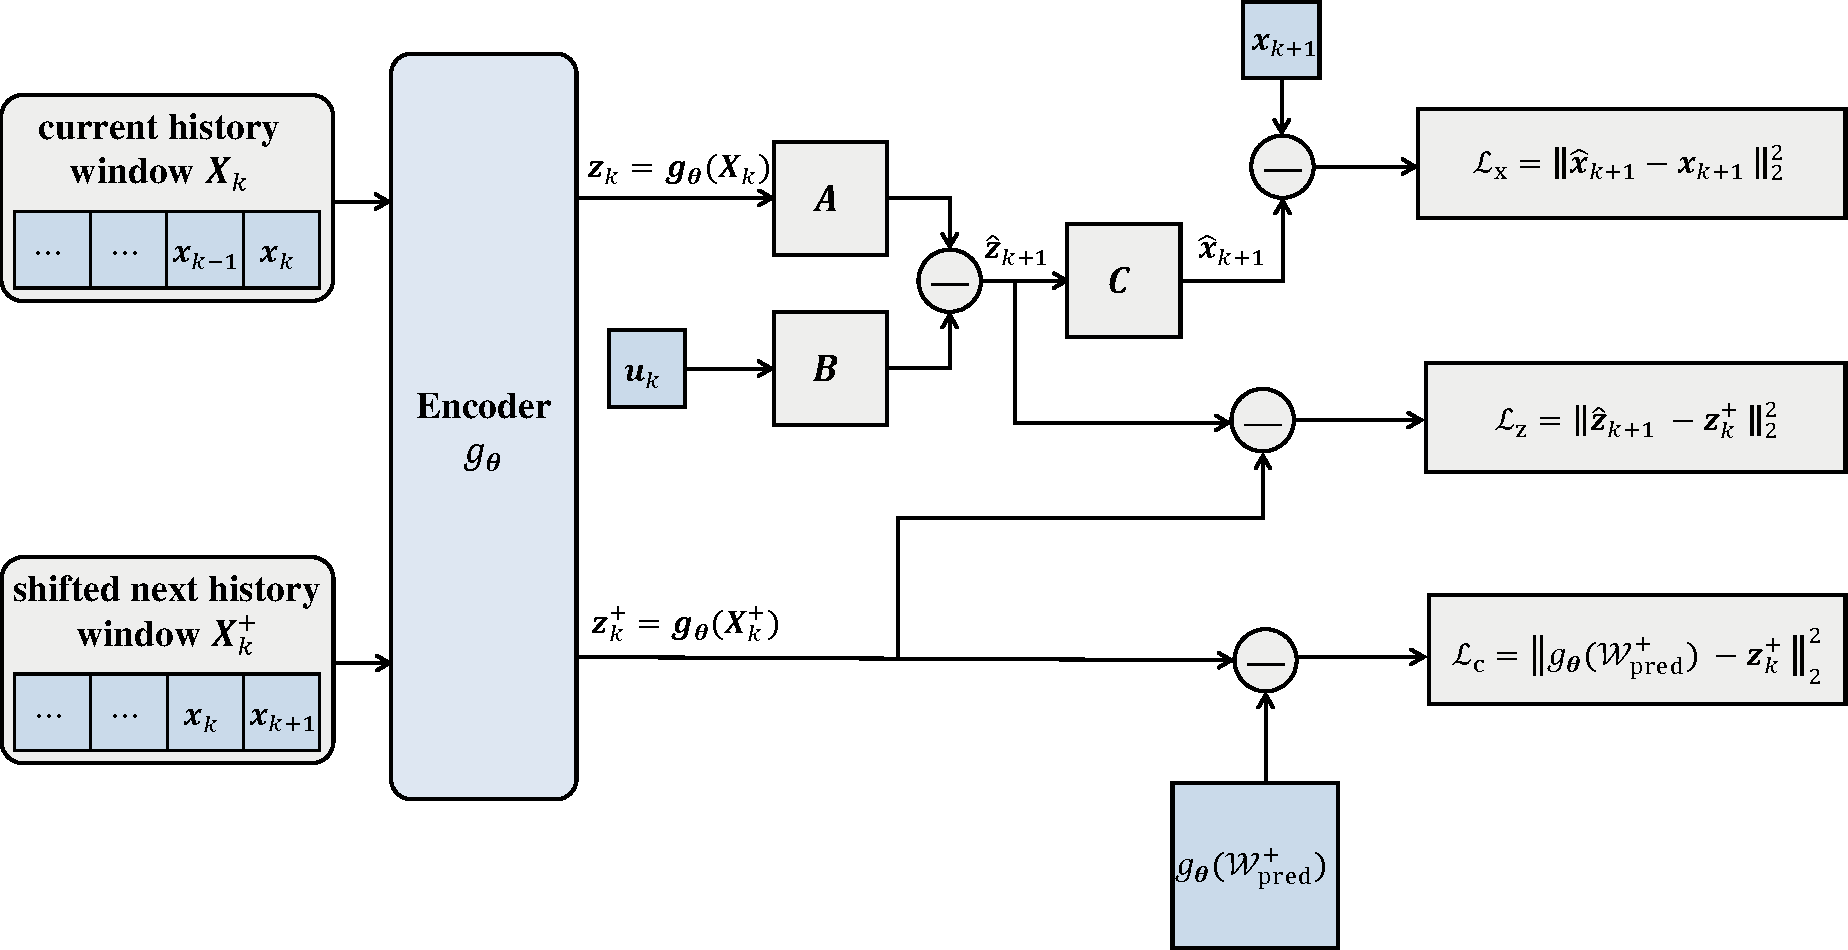
\includegraphics[width=0.95\linewidth]{pictures/Figure2.pdf}
    \caption{Stage~1 training procedure. The current history window 
    $\mX_k$ and the shifted window $\mX_k^{+}$ are each encoded by 
    $g_\theta$ to produce $\vz_k$ and $\vz_k^{+}$. The linear model 
    $(\mA,\mB)$ generates the one-step prediction $\hat{\vz}_{k+1}$, 
    from which $\hat{\vx}_{k+1}$ is recovered via $\mC$. Three 
    consistency losses $\mathcal{L}_x$, $\mathcal{L}_z$, and 
    $\mathcal{L}_c$ jointly supervise the encoder and linear dynamics.}
    \label{fig:training_procedure}
\end{figure}

In Stage~2, the encoder parameters are fixed and all latent trajectories are recomputed over the dataset. The linear dynamics are then re-estimated in closed form using ridge-regularized EDMD,
\begin{equation}
    \mTheta^{*} = (\mZ^{+})^\top \mOmega \left(\mOmega^\top \mOmega + \lambda \mI\right)^{-1},
\end{equation}
from which $\mA^{*}$ and $\mB^{*}$ are extracted. This refitting stage enforces consistency between the learned representation and the optimal linear regression solution, improving numerical stability and prediction accuracy. For notational simplicity, we overwrite $(\mA,\mB)\leftarrow(\mA^{*},\mB^{*})$ and use $(\mA,\mB)$ to denote the final refitted matrices in the remainder of the paper.

After training, the model is deployed autoregressively for multi-step prediction. Starting from an initial history window $\mX_0$, the lifted state is computed as $\vz_k = g_\theta(\mX_k)$ and propagated according to
\begin{equation}
    \hat{\vz}_{k+1} = \mA \vz_k + \mB \vu_k, \qquad
    \hat{\vx}_{k+1} = \mC \hat{\vz}_{k+1}.
\end{equation}
The history window is updated by appending $\hat{\vx}_{k+1}$ and discarding the oldest state. This rollout mechanism is used for evaluation in Section~\ref{sec:experiments}.

\begin{algorithm}[!t]
\caption{Transformer-Koopman Training Algorithm}
\label{alg:training}
\begin{algorithmic}[1]

\STATE \textbf{Input:} Dataset $\mathcal{D}$ \eqref{eq:dataset};
$P, p, d, \lambda_x, \lambda_z, \lambda_c, \lambda, E$

\STATE \textbf{Output:} Encoder $\theta^{*}$; matrices $\mA^{*}, \mB^{*}$

\STATE \textbf{Stage~0:}
Initialize $\theta$ randomly; encode $\mathcal{D}$ to obtain
$\mZ$, $\mZ^{+}$, $\mU$; compute $(\mA,\mB)$ via \eqref{eq:edmd_solution}.

\vspace{2pt}

\STATE \textbf{Stage~1:}
\FOR{epoch $\ell = 1$ \TO $E$}
    \FOR{each mini-batch $\mathcal{B} \subset \mathcal{D}$}
        \STATE Compute $\mathcal{L}_{\mathrm{pre}}$
               via \eqref{eq:loss_x}--\eqref{eq:pretraining_loss}.
        \STATE Update $(\theta, \mA, \mB)$ via gradient descent.
    \ENDFOR
\ENDFOR

\vspace{2pt}

\STATE \textbf{Stage~2:}
Fix $\theta^{*}$; recompute $\mZ$, $\mZ^{+}$, $\mU$;
obtain $(\mA^{*}, \mB^{*})$ via \eqref{eq:edmd_solution}.

\RETURN $\theta^{*}, \mA^{*}, \mB^{*}$

\end{algorithmic}
\end{algorithm}

% ---------------------------------------------------------
\subsection{Modeling Error Characterization}
\label{subsec:modeling_error}
% ---------------------------------------------------------

The identified lifted dynamics are approximate due to finite-dimensional Koopman truncation and encoder approximation error. We define the one-step modeling residual as
\begin{equation}
    \vw_k = \vz_{k+1} - (\mA \vz_k + \mB \vu_k),
    \label{eq:modeling_error}
\end{equation}
where $\vz_{k+1} = g_\theta(\mX_{k+1})$. In general, $\vw_k \neq \mathbf{0}$ even after training. When the state and control input remain within compact sets, the Koopman approximation error is theoretically bounded \cite{korda2018linear}. In practice, the bound $\varepsilon$ can be estimated by evaluating the one-step prediction residual on a held-out validation set.

% =========================================================
\section{Controller Design and Stability Analysis}
\label{sec:control}
% =========================================================

In this section, we develop a tracking controller based on the identified Koopman model and analyze the resulting closed-loop system.

% ---------------------------------------------------------
\subsection{Controller Design}
\label{subsec:controller_design}
% ---------------------------------------------------------

Based on the identified lifted dynamics \eqref{eq:temporal_dynamics} and the structured lifted state \eqref{eq:lifted_state_form}, we design a tracking controller in the lifted space. Let $\{\vx_k^{\mathrm{ref}}\}$ denote a reference state trajectory, and define the corresponding lifted reference trajectory as
\begin{equation}
    \vz_k^{\mathrm{ref}} = [\vx_k^{\mathrm{ref}};\,\vh_k^{\mathrm{ref}}],
    \label{eq:lifted_reference}
\end{equation}
where $\vh_k^{\mathrm{ref}}$ is obtained by encoding the reference history window. The lifted tracking error is then defined as
\begin{equation}
    \ve_k^z = \vz_k - \vz_k^{\mathrm{ref}}
    =
    \begin{bmatrix}
        \ve_k^x \\ \ve_k^h
    \end{bmatrix}
    =
    \begin{bmatrix}
        \vx_k - \vx_k^{\mathrm{ref}} \\
        \vh_k - \vh_k^{\mathrm{ref}}
    \end{bmatrix}.
    \label{eq:structured_error}
\end{equation}

We decompose the control input into feedforward and feedback terms,
\begin{equation}
    \vu_k = \vu_{\mathrm{ff},k} + \vu_{\mathrm{fb},k}.
    \label{eq:control_decomposition}
\end{equation}
The feedforward term compensates for the nominal reference evolution in the lifted space and is chosen as
\begin{equation}
    \vu_{\mathrm{ff},k}
    =
    \mB^\dagger \!\left(\vz_{k+1}^{\mathrm{ref}} - \mA \vz_k^{\mathrm{ref}}\right),
    \label{eq:feedforward}
\end{equation}
where $\mB^\dagger$ denotes the Moore--Penrose pseudoinverse of $\mB$.

The feedback term is designed from the structured lifted error as
\begin{equation}
    \vu_{\mathrm{fb},k}
    =
    -\mK_x \ve_k^x - \mK_h \ve_k^h
    =
    -\mK_c \ve_k^z,
    \label{eq:hierarchical_fb}
\end{equation}
where $\mK_c = [\mK_x\;|\;\mK_h]$ is partitioned according to \eqref{eq:structured_error}. To determine $\mK_c$, we perform a discrete-time LQR design for the pair $(\mA,\mB)$ with cost
\begin{equation}
    J = \sum_{k=0}^{\infty}
    \left[
        (\ve_k^z)^\top \mQ\,\ve_k^z
        +
        (\vu_{\mathrm{fb},k})^\top \mR\,\vu_{\mathrm{fb},k}
    \right],
    \label{eq:lqr_objective}
\end{equation}
where $\mR \succ \mathbf{0}$ and
\begin{equation}
    \mQ =
    \begin{bmatrix}
        \mQ_x & \mathbf{0} \\
        \mathbf{0} & \alpha \mQ_h
    \end{bmatrix},
    \qquad \alpha \in [0,1),
    \label{eq:block_diag_Q}
\end{equation}
with $\mQ_x \succ \mathbf{0}$ and $\mQ_h \succ \mathbf{0}$. Here, $\mQ_x$ determines the primary tracking objective in the physical state, whereas $\alpha \mQ_h$ assigns a smaller auxiliary penalty to the feature error. In practice, $\mQ_x$ is chosen dominant and $\alpha$ is set small, with $\alpha = 0$ also admissible if no explicit penalty on $\ve_k^h$ is desired. Solving the standard discrete-time Riccati equation yields
\begin{equation}
    \mK_c
    =
    (\mR + \mB^\top \mP \mB)^{-1} \mB^\top \mP \mA
    =
    [\mK_x\;|\;\mK_h].
    \label{eq:lqr_gain}
\end{equation}

Combining \eqref{eq:control_decomposition}--\eqref{eq:hierarchical_fb}, the resulting control law is
\begin{equation}
    \vu_k
    =
    \mB^\dagger \!\left(\vz_{k+1}^{\mathrm{ref}} - \mA \vz_k^{\mathrm{ref}}\right)
    - \mK_c \ve_k^z.
    \label{eq:full_ctrl}
\end{equation}

The overall controller structure is illustrated in Fig.~\ref{fig:control_architecture}.

\begin{figure}[!t]
    \centering
    %\includegraphics[width=0.9\linewidth]{figs/fig2_control_architecture.pdf}
    \caption{Control architecture based on the structured lifted state $\vz_k=[\vx_k;\vh_k]$. The reference trajectory is encoded to $\vz_k^{\mathrm{ref}}=[\vx_k^{\mathrm{ref}};\vh_k^{\mathrm{ref}}]$, and the current state history is encoded to $\vz_k=[\vx_k;\vh_k]$. The error $\ve_k^z = \vz_k - \vz_k^{\mathrm{ref}}$ drives both feedforward and feedback control terms.}
    \label{fig:control_architecture}
\end{figure}

% ---------------------------------------------------------
\subsection{Stability Analysis}
\label{subsec:stability}
% ---------------------------------------------------------

We analyze the closed-loop tracking error induced by the control law \eqref{eq:full_ctrl} applied to the identified Koopman model.

\begin{theorem}[Ultimate Boundedness of Tracking Error]
\label{thm:ub}
Consider the lifted dynamics \eqref{eq:temporal_dynamics} under the control law \eqref{eq:full_ctrl}. Suppose that $(\mA, \mB)$ is stabilizable, $(\mA, \mQ^{1/2})$ is detectable, and the modeling residual satisfies $\|\vw_k\| \leq \varepsilon$ for all $k \geq 0$. Then the closed-loop system achieves ultimately uniformly bounded tracking; that is, the lifted tracking error satisfies
\begin{equation}
    \|\ve_k^z\| \leq \frac{\varepsilon}{1 - \|\mA_{\mathrm{cl}}\|}
    \label{eq:ub_bound}
\end{equation}
for all sufficiently large $k$, and consequently
\begin{equation}
    \|\vx_k - \vx_k^{\mathrm{ref}}\| \leq \frac{\varepsilon}{1 - \|\mA_{\mathrm{cl}}\|}.
    \label{eq:phys_bound}
\end{equation}
\end{theorem}

\begin{proof}
Substituting \eqref{eq:full_ctrl} into \eqref{eq:temporal_dynamics} and using \eqref{eq:modeling_error}, the tracking error $\ve_k^z = \vz_k - \vz_k^{\mathrm{ref}}$ evolves as
\begin{equation}
    \ve_{k+1}^z = \mA_{\mathrm{cl}}\, \ve_k^z + \vw_k,
    \label{eq:cl_error_dyn}
\end{equation}
where $\mA_{\mathrm{cl}} = \mA - \mB\mK_c$. By the stabilizability and detectability assumptions and standard LQR theory, $\mA_{\mathrm{cl}}$ is Schur stable with $\|\mA_{\mathrm{cl}}\| < 1$. Iterating \eqref{eq:cl_error_dyn} and applying the triangle inequality, the bound \eqref{eq:ub_bound} follows from the convergence of the geometric series $\sum_{i=0}^{\infty}\|\mA_{\mathrm{cl}}\|^i$. The physical-state bound \eqref{eq:phys_bound} follows from $\|\vx_k - \vx_k^{\mathrm{ref}}\| = \|\mC\ve_k^z\| \leq \|\ve_k^z\|$ since $\|\mC\| = 1$.
\end{proof}

The ultimate bound scales linearly with the modeling residual $\varepsilon$: improving the Koopman approximation accuracy directly tightens the closed-loop tracking guarantee, and as $\varepsilon \to 0$, the tracking error converges to zero asymptotically.

% =========================================================
\section{Experiments}
\label{sec:experiments}
% =========================================================

We evaluate the proposed method on two controlled-system datasets, focusing on open-loop trajectory prediction and architectural ablations. In addition, we outline a planned closed-loop trajectory-tracking validation based on the learned Koopman models.

\subsection{Experimental Setup}

\subsubsection{Datasets}

Experiments are conducted on two real-world systems with different state and input dimensions. The first platform is a \textbf{6-DoF manipulator system (Geomagic Touch)} with a 6-dimensional state and 3 control inputs. The dataset contains 15 training trajectories, 4 validation trajectories, and 1 test trajectory, comprising 74,655, 19,909, and 4,976 time steps, respectively. The second platform is a \textbf{soft robotic system} with a 2-dimensional state and 2 control inputs. The dataset consists of 49 training trajectories, 21 validation trajectories, and 1 test trajectory, with 24,150, 10,351, and 500 time steps, respectively. In both datasets, training samples are constructed from history windows that remain within individual trajectories. State and control inputs are normalized using statistics computed from the training set and applied consistently to validation and test data.

\subsubsection{Compared Methods}

We compare three Koopman-based models under a unified evaluation pipeline: (i)~\textbf{EDMD}, a classical Koopman approximation with hand-crafted observables; (ii)~\textbf{MLP-Koopman}, a learned lifting map based on an MLP encoder using instantaneous states; and (iii)~\textbf{Transformer-Koopman}, the proposed temporal lifting model based on history windows and patch-based Transformer encoding.

\subsubsection{Evaluation Protocol}
\label{sec:eval_protocol}

All models are evaluated using open-loop autoregressive rollout. Each rollout is initialized with a ground-truth history window from the test trajectory. At each step, $\hat{\vx}_{k+1} = \mC(\mA \vz_k + \mB \vu_k)$ with $\vz_k = g_\theta(\mX_k)$, and the history window is updated by appending $\hat{\vx}_{k+1}$ and removing the oldest state. Performance is measured using trajectory-level RMSE and MAE over the rollout horizon.

\subsection{Trajectory Prediction Accuracy}

We first compare trajectory-prediction performance across all methods. Table~\ref{tab:prediction_platform_a} reports results on the 6-DoF manipulator system. Learned liftings significantly outperform hand-crafted observables, and incorporating temporal context through the proposed method further improves prediction accuracy, indicating that short-term temporal correlations, when explicitly encoded, lead to more accurate linear latent dynamics under autoregressive rollout.

\begin{table}[!t]
\renewcommand{\arraystretch}{1.2}
\caption{Open-loop trajectory prediction on the 6-DoF manipulator system}
\label{tab:prediction_platform_a}
\centering
\begin{tabular}{lcc}
\toprule
Method & RMSE & MAE \\
\midrule
EDMD & 2.6206 & 1.9544 \\
MLP-Koopman & 0.5074 & 0.2511 \\
Transformer-Koopman & \textbf{0.1768} & \textbf{0.0917} \\
\bottomrule
\end{tabular}
\end{table}

\subsection{Ablation Study}

We next evaluate the effect of architectural components on the soft robotic system. The best-performing configuration uses $P=6$, $p=2$, $d=8$, $d_{\mathrm{model}}=16$, three Transformer layers ($L=3$), two attention heads ($n_h=2$), and EDMD regularization $\lambda=10^{-4}$.

\begin{table}[!t]
\renewcommand{\arraystretch}{1.2}
\caption{Ablation results on the soft robotic system}
\label{tab:ablation_platform_b}
\centering
\begin{tabular}{p{0.62\columnwidth}c}
\toprule
Variant & Test RMSE \\
\midrule
Best setting ($P=6$, $p=2$) & \textbf{0.01408} \\
$P=4$ & 0.01525 \\
$P=2$ & 0.01710 \\
$P=2$, $p=1$ (no patching) & 0.03362 \\
1 layer, 1 head & 0.01513 \\
Larger model ($d=16$) & 0.01481 \\
$\lambda=1$ & 0.01591 \\
$\lambda=10$ & 0.02153 \\
\bottomrule
\end{tabular}
\end{table}

Reducing the history length degrades performance, confirming the importance of temporal context. Removing patch-based tokenization ($p=1$) leads to a substantial performance drop, indicating that local temporal aggregation is critical. Increasing model size does not yield consistent improvements, suggesting that compact representations are sufficient once the relevant temporal features are captured. Strong regularization deteriorates performance, whereas moderate regularization stabilizes the regression.

\subsection{Planned Trajectory-Tracking Validation}

We finally outline a closed-loop trajectory-tracking validation using the controller in Section~\ref{sec:control}, to be conducted on the soft robotic system. The controller structure will be fixed across all models, while only the learned Koopman representation is varied, thereby isolating the effect of model quality on tracking performance. Evaluation metrics will include tracking RMSE, peak error, and control effort.

% =========================================================
\section{Conclusion}
\label{sec:conclusion}
% =========================================================

This paper presented Transformer-Koopman, a temporal lifting framework for learning Koopman models of controlled nonlinear systems from finite history windows. The framework is organized around three coupled technical decisions. First, a finite history window of recent states is used as encoder input rather than the instantaneous state alone, because single-time-step snapshots discard the short-term temporal correlations among successive states that are informative for constructing an accurate linear latent evolution law. Second, the history window is encoded by a Transformer with non-overlapping temporal patch tokenization: patch tokenization aggregates locally correlated time steps before global modeling, and self-attention then captures pairwise temporal dependencies across patches without the sequential bottleneck of recurrent architectures. Third, the encoder output is integrated with the current physical state into a compact fixed-dimensional lifted vector, which is directly compatible with the Koopman requirement of finite-dimensional linear dynamics and provides exact physical-state recovery through a fixed projection, avoiding a learned nonlinear decoder and preserving a clean interface for controller design.

The completed experiments support the main identification claim of the paper. On both experimental platforms, the proposed method achieves substantially lower rollout error than EDMD and MLP-Koopman baselines, consistent with the hypothesis that encoding short-term temporal correlations in the lifting map improves Koopman approximation accuracy. The ablation studies confirm that temporal context, patch design, and moderate regularization each contribute meaningfully to model quality, and that removing any of these ingredients degrades performance in ways that align with their intended roles in the design. The improvement in modeling residual $\varepsilon$ translates, through the stability analysis of Section~\ref{sec:control}, into a tighter theoretical bound on closed-loop tracking error.

Closed-loop tracking validation is not yet included in the present manuscript. The most direct next step is therefore to compare the learned predictors under a common controller structure and assess whether improved predictive accuracy also translates into improved control performance. A second natural extension is to study richer lifting inputs, including joint state-input histories, within the same control-oriented Koopman framework.

\begin{thebibliography}{99}

\bibitem{koopman1931hamiltonian}
B. O. Koopman, ``Hamiltonian systems and transformation in Hilbert space,'' \emph{Proc. Natl. Acad. Sci. USA}, vol. 17, no. 5, pp. 315--318, 1931.

\bibitem{koopman1932spectra}
B. O. Koopman and J. von Neumann, ``Dynamical systems of continuous spectra,'' \emph{Proc. Natl. Acad. Sci. USA}, vol. 18, no. 3, pp. 255--263, 1932.

\bibitem{mezic2005spectral}
I. Mezi\'c, ``Spectral properties of dynamical systems, model reduction and decompositions,'' \emph{Nonlinear Dyn.}, vol. 41, pp. 309--325, 2005.

\bibitem{ljung1999system}
L. Ljung, \emph{System Identification: Theory for the User}, 2nd ed. Upper Saddle River, NJ, USA: Prentice Hall, 1999.

\bibitem{vanoverschee1994n4sid}
P. Van Overschee and B. De Moor, ``N4SID: Subspace algorithms for the identification of combined deterministic-stochastic systems,'' \emph{Automatica}, vol. 30, no. 1, pp. 75--93, 1994.

\bibitem{nelles2020nonlinear}
O. Nelles, \emph{Nonlinear System Identification: From Classical Approaches to Neural Networks and Fuzzy Models}, 2nd ed. Cham, Switzerland: Springer, 2020.

\bibitem{rowley2009spectral}
C. W. Rowley, I. Mezi\'c, S. Bagheri, P. Schlatter, and D. S. Henningson, ``Spectral analysis of nonlinear flows,'' \emph{J. Fluid Mech.}, vol. 641, pp. 115--127, 2009.

\bibitem{williams2015data}
M. O. Williams, I. G. Kevrekidis, and C. W. Rowley, ``A data--driven approximation of the Koopman operator: Extending dynamic mode decomposition,'' \emph{J. Nonlinear Sci.}, vol. 25, no. 6, pp. 1307--1346, 2015.

\bibitem{williams2015kernel}
M. O. Williams, C. W. Rowley, and I. G. Kevrekidis, ``A kernel-based method for data-driven Koopman spectral analysis,'' \emph{J. Comput. Dyn.}, vol. 2, no. 2, pp. 247--265, 2015.

\bibitem{arbabi2017ergodic}
H. Arbabi and I. Mezi\'c, ``Ergodic theory, dynamic mode decomposition, and computation of spectral properties of the Koopman operator,'' \emph{SIAM J. Appl. Dyn. Syst.}, vol. 16, no. 4, pp. 2096--2126, 2017.

\bibitem{brunton2022modern}
S. L. Brunton, M. Budi\v{s}i\'c, E. Kaiser, and J. N. Kutz, ``Modern Koopman theory for dynamical systems,'' \emph{SIAM Rev.}, vol. 64, no. 2, pp. 229--340, 2022.

\bibitem{otto2021koopman}
S. E. Otto and C. W. Rowley, ``Koopman operators for estimation and control of dynamical systems,'' \emph{Annu. Rev. Control Robot. Auton. Syst.}, vol. 4, pp. 59--87, 2021.

\bibitem{takeishi2017koopman}
N. Takeishi, Y. Kawahara, and T. Yairi, ``Learning Koopman invariant subspaces for dynamic mode decomposition,'' in \emph{Proc. NeurIPS}, 2017, pp. 1130--1140.

\bibitem{yeung2019learning}
E. Yeung, S. Kundu, and N. Hodas, ``Learning deep neural network representations for Koopman operators of nonlinear dynamical systems,'' in \emph{Proc. ACC}, 2019, pp. 4832--4839.

\bibitem{lusch2018deep}
B. Lusch, J. N. Kutz, and S. L. Brunton, ``Deep learning for universal linear embeddings of nonlinear dynamics,'' \emph{Nat. Commun.}, vol. 9, no. 1, p. 4950, 2018.

\bibitem{morton2019deep}
J. Morton, F. D. Witherden, and M. J. Kochenderfer, ``Deep variational Koopman models: Inferring Koopman observations for uncertainty-aware dynamics modeling and control,'' in \emph{Proc. IJCAI}, 2019, pp. 5113--5119.

\bibitem{azencot2020forecasting}
O. Azencot, N. B. Erichson, V. Lin, and M. W. Mahoney, ``Forecasting sequential data using consistent Koopman autoencoders,'' in \emph{Proc. ICML}, 2020, pp. 475--485.

\bibitem{yuan2022variational}
J. Yuan, A. A. Heydari, and Z. Zhang, ``Variational Koopman models: Slow coherent structures and uncertainty quantification,'' \emph{IEEE Trans. Autom. Control}, vol. 67, no. 11, pp. 5905--5920, 2022.

\bibitem{otto2019linearly}
S. E. Otto and C. W. Rowley, ``Linearly-recurrent autoencoder networks for learning dynamics,'' \emph{SIAM J. Appl. Dyn. Syst.}, vol. 18, no. 1, pp. 558--593, 2019.

\bibitem{rank2019recurrent}
M. Rank, A. G. Georgescu, and S. Kirchner, ``Recurrent Koopman operator for data-driven modeling of nonlinear dynamics,'' \emph{IEEE Control Syst. Lett.}, vol. 3, no. 4, pp. 912--917, 2019.

\bibitem{forgione2021dynonet}
M. Forgione and D. Varagnolo, ``DynoNet: A neural network architecture for learning dynamical systems,'' \emph{Int. J. Adapt. Control Signal Process.}, vol. 35, no. 4, pp. 612--629, 2021.

\bibitem{brunton2016sindy}
S. L. Brunton, J. L. Proctor, and J. N. Kutz, ``Discovering governing equations from data by sparse identification of nonlinear dynamical systems,'' \emph{Proc. Natl. Acad. Sci. USA}, vol. 113, no. 15, pp. 3932--3937, 2016.

\bibitem{proctor2016dmdc}
J. L. Proctor, S. L. Brunton, and J. N. Kutz, ``Dynamic mode decomposition with control,'' \emph{SIAM J. Appl. Dyn. Syst.}, vol. 15, no. 1, pp. 142--161, 2016.

\bibitem{proctor2018generalizing}
J. L. Proctor, S. L. Brunton, and J. N. Kutz, ``Generalizing Koopman theory to allow for inputs and control,'' \emph{SIAM J. Appl. Dyn. Syst.}, vol. 17, no. 1, pp. 909--930, 2018.

\bibitem{brunton2016invariant}
S. L. Brunton, B. W. Brunton, J. L. Proctor, and J. N. Kutz, ``Koopman invariant subspaces and finite linear representations of nonlinear dynamical systems for control,'' \emph{PLOS ONE}, vol. 11, no. 2, e0150171, 2016.

\bibitem{korda2018linear}
M. Korda and I. Mezi\'c, ``Linear predictors for nonlinear dynamical systems: Koopman operator meets model predictive control,'' \emph{Automatica}, vol. 93, pp. 149--160, 2018.

\bibitem{han2020deep}
Y. Han, W. Hao, and U. Vaidya, ``Deep learning of Koopman representation for control,'' arXiv:2010.07546, 2020.

\bibitem{shi2022deep}
H. Shi and M. Q.-H. Meng, ``Deep Koopman operator with control for nonlinear systems,'' \emph{IEEE Robot. Autom. Lett.}, vol. 7, no. 3, pp. 7700--7707, 2022.

\bibitem{strasser2026overview}
R. Str\"asser, K. Worthmann, I. Mezi\'c, J. Berberich, M. Schaller, and F. Allg\"ower, ``An overview of Koopman-based control: From error bounds to closed-loop guarantees,'' \emph{Annu. Rev. Control}, vol. 61, art. 101035, 2026.

\bibitem{duran2025control}
J. F. Dur\'an-Sig\"uenza, L. I. Minchala, L. E. Garza-Casta\~n\'on, and H. Zhang, ``Control based on the Koopman operator: A comprehensive review,'' \emph{J. Franklin Inst.}, vol. 362, no. 18, art. 108256, 2025.

\bibitem{klus2018data}
S. Klus, P. Koltai, and C. Sch\"utte, ``Data-driven model reduction and transfer operator approximation,'' \emph{J. Nonlinear Sci.}, vol. 28, no. 3, pp. 985--1010, 2018.

\bibitem{vaswani2017attention}
A. Vaswani \emph{et al.}, ``Attention is all you need,'' in \emph{Proc. NeurIPS}, 2017, pp. 5998--6008.

\bibitem{zhou2021informer}
H. Zhou \emph{et al.}, ``Informer: Beyond efficient Transformer for long sequence time-series forecasting,'' in \emph{Proc. AAAI}, 2021, pp. 11106--11115.

\bibitem{wu2021autoformer}
H. Wu, J. Xu, J. Wang, and M. Long, ``Autoformer: Decomposition Transformers with auto-correlation for long-term series forecasting,'' in \emph{Proc. NeurIPS}, 2021, pp. 22419--22430.

\bibitem{zhou2022fedformer}
T. Zhou \emph{et al.}, ``FEDformer: Frequency enhanced decomposed Transformer for long-term series forecasting,'' in \emph{Proc. ICML}, 2022, pp. 27268--27286.

\bibitem{nie2023time}
Y. Nie, N. H. Nguyen, P. Sinthong, and J. Kalagnanam, ``A time series is worth 64 words: Long-term forecasting with Transformers,'' in \emph{Proc. ICLR}, 2023.

\bibitem{zeng2023transformers}
A. Zeng, M. Chen, L. Zhang, and Q. Xu, ``Are Transformers effective for time series forecasting?,'' in \emph{Proc. AAAI}, 2023, pp. 11121--11128.

\bibitem{liu2024itransformer}
Y. Liu \emph{et al.}, ``iTransformer: Inverted Transformers are effective for time series forecasting,'' in \emph{Proc. ICLR}, 2024.

\bibitem{forootani2026compact}
A. Forootani and M. Khosravi, ``Compact transformer variants for synthetic time series forecasting,'' \emph{Neurocomputing}, vol. 677, art. 133140, 2026.

\bibitem{forootani2025synthetic}
A. Forootani and M. Khosravi, ``Synthetic time series forecasting with Transformer architectures: Extensive simulation benchmarks,'' arXiv:2505.20048, 2025.

\bibitem{forootani2026deepkoopformer}
A. Forootani, M. Khosravi, and M. Barati, ``DeepKoopFormer: A Koopman enhanced Transformer based architecture for time series forecasting,'' \emph{npj Artif. Intell.}, vol. 2, art. 35, 2026.

\bibitem{forootani2026spectral}
A. Forootani and R. Iervolino, ``Learnable Koopman-enhanced Transformer-based time series forecasting with spectral control,'' arXiv:2602.02592, 2026.

\bibitem{wang2020linformer}
S. Wang, B. Z. Li, M. Khabsa, H. Fang, and H. Ma, ``Linformer: Self-attention with linear complexity,'' arXiv:2006.04768, 2020.

\bibitem{katharopoulos2020transformers}
A. Katharopoulos, A. Vyas, N. Pappas, and F. Fleuret, ``Transformers are RNNs: Fast autoregressive Transformers with linear attention,'' in \emph{Proc. ICML}, 2020, pp. 5156--5165.

\bibitem{choromanski2021performer}
K. M. Choromanski \emph{et al.}, ``Rethinking attention with Performers,'' in \emph{Proc. ICLR}, 2021.

\end{thebibliography}

\end{document}